\documentclass[12pt,letterpaper,twoside]{article}

\newif\ifsolution\solutiontrue   % Include the solutions
%\newif\ifsolution\solutionfalse  % Exclude the solutions

\usepackage{cme213}
\usepackage{xcolor}
\usepackage{float}
\usepackage{graphicx}

\newcommand{\T}[1]{\text{\texttt{#1}}}
\newcommand{\V}[1]{\text{\textit{#1}}}

\begin{document}

{\centering \textbf{Final Report: Neural Networks on CUDA\\}}
\vspace*{-8pt}\noindent\rule{\linewidth}{1pt}

Goal of the final project is to implement a neural network with parallel
matrix-matrix operations across four GPUs. Our neural network will be used
to identify images of hand-written digits from the MNIST dataset.

\paragraph{Section 1: Accelerated Matrix Multiplication} Idea: parallelize our generalized
in-place matrix mulitplication (GEMM) $C = \alpha*A*B + \beta*C$ across cores of one GPU. We
will be able to use this to excute multiple steps in the neural network's feed forward
and back propagation operations.

\begin{itemize}
    \item \textbf{Algorithm \#1:} Our first (naive) implementation is correct but
    very inefficient. We ask each thread to compute a single value of the output matrix
    C. This requires each thread to fetch from global memory an entire row of matrix A
    and column from matrix B, resulting in a lot of repeated global memory requests
    for the same information. Note, Algorithm 1 was used for part 1 of the project.

    \item \textbf{Algorithm \#2:} Our second implementation makes use of shared
    memory, which affords us increased bandwidth. In particular, algorithm 2
    loads a 32x32 block from matrix A and matrix B into shared memory before
    performing a partial update on the corresponding 32x32 block of output
    matrix C. Each thread still only performs an update for a single cell
    in the output matrix.

    \item \textbf{Algorithm \#3: } Our third implementation uses a specific
    thread block of size 4x16 to compute a partial update of a 64x16 block of
    output matrix C. Each thread in this case updates one 1x16 row of this
    64x16 block, which reduces latency and increases overall arithmetic intensity
    compared to algorithms 1 and 2. This implementation makes use of shared memory
    as well as local (register) memory.

\end{itemize}

\begin{figure}[!htbp]
    \centering
    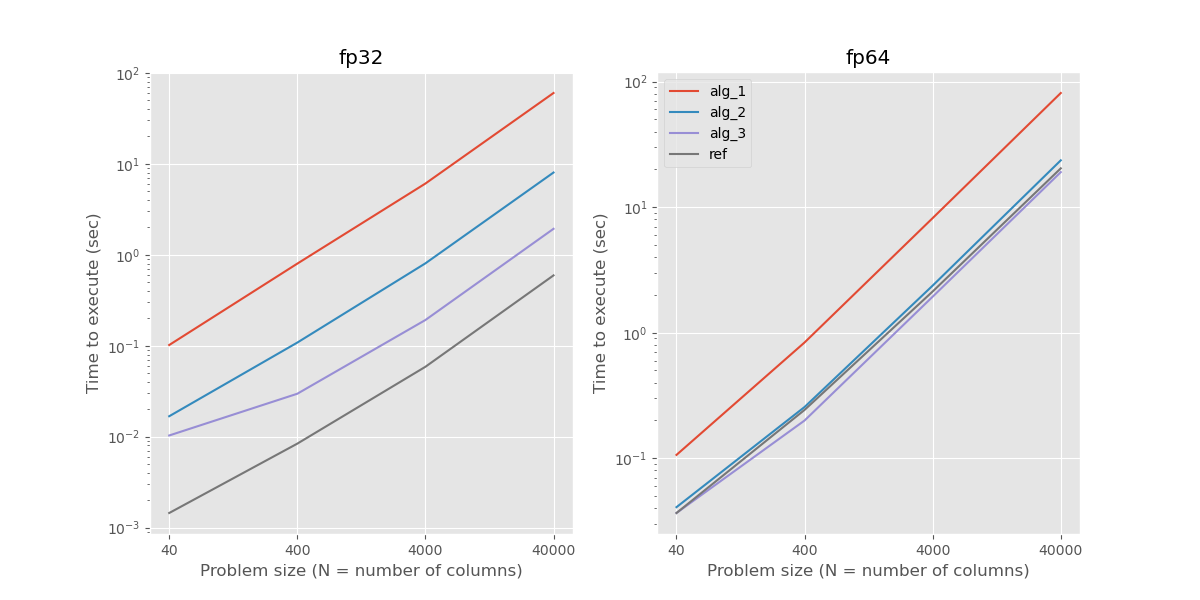
\includegraphics[scale=0.6]{speed_alg_vs_problem_size.png}
    \caption{Speed test of GEMM algorithms for float and double precision}
\end{figure}

In Figure 1, we can see that our algorithms progressively improve towards
(but do not match) the reference cublas solution for FP32 numbers. However,
for double precision FP64 numbers, algorithms 2, 3 and the reference all
perform similarly, with algorithm 3 actually surpassing the reference.
This is likely because the cublas solution is optimized for FP32 given
most use cases (e.g. neural network training) do not require double
precision.

\begin{figure}[!htbp]
    \centering
    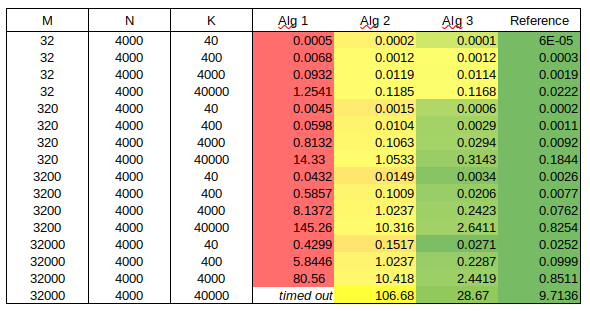
\includegraphics[scale=0.7]{speed_alg_vs_dimensions.png}
    \caption{Speed test of GEMM algorithms for different M x N dimensions}
\end{figure}

Figure 2 shows a heat map with speed tests for different GEMM matrix dimension
combinations (assuming FP32). Since algorithm 1 $<$ algorithm 2 $<$ algorithm 3
$<$ reference for all settings, I have consistenly implemented algorithm 3
throughout my neural network kernels. It is intersting to note that this
relative differences shift quite a bit, but never enough to justify
a change of algorithm for specific settings. Further analysis could take
into account other input parameter options such as size of thread block,
number of processes, etc.

\textbf{GEMM correctness.} See grading output below from GEMM Algorithm 3. Our
results match \texttt{cublas\_gemm} values to within precision error for
FP32 numbers (rel difference of $10^{-7}$). This is consistent across test
cases.

\begin{verbatim}
*** Grading mode 4 ***

main -g 4
Number of MPI processes = 1
Number of CUDA devices = 4

Entering GEMM Benchmarking mode! Stand by.

Starting GEMM 1: M = 3200; N = 4000; K = 3136
GEMM matched with reference successfully! Rel diff = 1.00042e-07
Time for reference GEMM implementation: 0.0690576 seconds
Time for my GEMM implementation: 0.21447 seconds
Completed GEMM 1

Starting GEMM 2: M = 3200; N = 400; K = 4000
GEMM matched with reference successfully! Rel diff = 4.57243e-07
Time for reference GEMM implementation: 0.00814952 seconds
Time for my GEMM implementation: 0.0293013 seconds
Completed GEMM 2

Starting GEMM 3: M = 3200; N = 40; K = 4000
GEMM matched with reference successfully! Rel diff = 7.29707e-07
Time for reference GEMM implementation: 0.00140982 seconds
Time for my GEMM implementation: 0.0101932 seconds
Completed GEMM 3

*** Tests are complete ***
\end{verbatim}

\pagebreak
\paragraph{Section 2: Parallelize Neural Network (Single GPU)} Idea: training a neural
network involves repeatedly updating weights and biases at each layer through forward
and backwards propagation. Internally, these operations are mostly various adaptations
of genralized matrix multiplication! We want to take existing sequential code and
parallelize each using our optimized GEMM algorithm from Section 1.

Based on profiling analysis from my part 1 of the project ('naive' version in table below),
I implemented a series of updates to improve the performance of my code.
\begin{table}[h]
    \begin{tabular}{llllll}
    \textbf{version} & \textbf{procs} & \textbf{mode\_1} & \textbf{mode\_2} & \textbf{mode\_3} &                                      \\
    naive            & 4              & 8.352            & 2.405            & 0.888            & project part 1 implementation        \\
    update\_1        & 4              & 6.420            & 2.026            & 0.694            & updated kernels to use algorithm 3   \\
    update\_2        & 4              & 6.218            & 1.989            & 0.664            & incorporated tranpose into kernels   \\
    update\_3        & 4              & 6.194            & 1.947            & 0.618            & combined gradient descent step       \\
    update\_4        & 4              & 6.129            & 1.947            & 0.622            & switched to in-place operations      \\
    reference        & 4              & 2.580            & 0.980            & 0.590            &
    \end{tabular}
\end{table}

\begin{itemize}
    \item \textbf{Update 1: GEMM Algorithms.} My generalized matrix multplication
    from part 1 was very inefficient: each thread computes just one output value
    and does not make use of shared memory. Algorithm 3 from Section 1 is an order
    of magnitude faster due to its use of shared memory and sophisticated memory
    access pattern (more coelesced). My first update was therefore to adapt all
    variations of GEMM used in our neural network training to use the Algorithm
    3 implementation.

    \item \textbf{Update 2: Tranpose Kernels.} My intial version of used
    additional memory and a dedicated kernel (\texttt{kernel\_transpose}) to
    perform the three matrix tranpose steps required in back propagation.
    While this was nicely modular and therefore useful for unit testing,
    it was inefficient. This second update eliminates the need to store
    \texttt{d\_XT}, \texttt{d\_a0T}, and \texttt{d\_W1T} in my cache (removing
    associated cuda malloc statements) and no longer requires three separate
    instantiations of the transpose kernel. I did this by simply writing
    additional GEMM kernel variants that handle transposing input matrices.

    \item \textbf{Update 3: Graident Descent.} My normalization, regularization
    and gradient descent steps all previously were implemented in separate kernels.
    It turns out that these steps can be readily combined and re-expressed together
    as the following matrix addition expression (e.g. for W[0]):

    $$W[0] \mathrel{{-}{=}} l*(\frac{1}{n} dW[0] + r W[0])$$.

    \item \textbf{Update 4: In-place Operations.} I allocate memory on the device for
    a bunch of temporary variables to assist with intermediate calculations during
    feed forward and back propagation steps. Looking at the profiler output, these
    malloc steps are quite expensive. I implemented updates to eliminate \texttt{z0},
    \texttt{z1}, \texttt{yc} and \texttt{1ma0} from my cache variables by overwriting
    existing cache variables where possible (e.g. sigmoid function can update a0 in-place).
\end{itemize}

Each update above resulted in a net improvement for the \texttt{mode 1} speed test at
N=4 processes. The increases were diminishing in magnitude, with \texttt{Update 1}
having the largest impact (25\%) and \texttt{Update 4} being almost within margin
of error given natural variability of icme gpu runtimes. The best result was 6.129
seconds for \texttt{mode 1} after \texttt{Update 4}.

\textbf{Neural Network correctness.} For all of the parameter variations tested, the
weights and biases produced by the parallel neural network training algorithm match
within machine accuracy the CPU sequential code (i.e. max and l2 norms differ
by $10^{-7}$). Furthermore, when tested using double precision floating point
numbers, our norm errors reduce to $O(10^{-16})$ as we would expect if the
differences were purely machine accuracy rather than logic inconsistencies.

\begin{verbatim}
* Mode 1 *
mpirun -np 3 /home/jelc/cme213-para/project/main -g 1
Number of MPI processes = 4
Number of CUDA devices = 4
num_neuron=100, reg=0.0001, learning_rate=0.0005, num_epochs=40, batch_size=800
Loading training data
Training data information:
Size of x_train, N =  60000
Size of label_train = 60000

Start Parallel Training
Time for Parallel Training: 6.12856 seconds
Precision on validation set for parallel training = 0.829167

Grading mode on. Now checking for correctness...

Max norm of diff b/w seq and par: W[0]: 1.70544e-07, b[0]: 1.02758e-06
l2  norm of diff b/w seq and par: W[0]: 1.94657e-07, b[0]: 6.68161e-07
Max norm of diff b/w seq and par: W[1]: 1.16507e-07, b[1]: 1.61697e-07
l2  norm of diff b/w seq and par: W[1]: 1.43914e-07, b[1]: 2.84616e-07

* Mode 2 *
mpirun -np 3 /home/jelc/cme213-para/project/main -g 2
Number of MPI processes = 4
Number of CUDA devices = 4
num_neuron=100, reg=0.0001, learning_rate=0.001, num_epochs=10, batch_size=800
Loading training data
Training data information:
Size of x_train, N =  60000
Size of label_train = 60000

Start Parallel Training
Time for Parallel Training: 1.94655 seconds
Precision on validation set for parallel training = 0.756

Grading mode on. Now checking for correctness...

Max norm of diff b/w seq and par: W[0]: 8.80379e-08, b[0]: 5.97242e-07
l2  norm of diff b/w seq and par: W[0]: 1.20557e-07, b[0]: 5.32801e-07
Max norm of diff b/w seq and par: W[1]: 1.03612e-07, b[1]: 2.44647e-07
l2  norm of diff b/w seq and par: W[1]: 1.2233e-07, b[1]: 2.04047e-07

* Mode 3 *
mpirun -np 3 /home/jelc/cme213-para/project/main -g 3
Number of MPI processes = 4
Number of CUDA devices = 4
num_neuron=100, reg=0.0001, learning_rate=0.002, num_epochs=1, batch_size=800
Loading training data
Training data information:
Size of x_train, N =  60000
Size of label_train = 60000

Start Parallel Training
Time for Parallel Training: 0.621657 seconds
Precision on validation set for parallel training = 0.463667

Grading mode on. Now checking for correctness...

Max norm of diff b/w seq and par: W[0]: 3.38911e-08, b[0]: 6.03991e-07
l2  norm of diff b/w seq and par: W[0]: 5.41403e-08, b[0]: 3.4692e-07
Max norm of diff b/w seq and par: W[1]: 5.75366e-08, b[1]: 4.68431e-07
l2  norm of diff b/w seq and par: W[1]: 7.41761e-08, b[1]: 3.59052e-07
\end{verbatim}

\textbf{Remarks on debgugging.} This step required significant debugging effort given
the inherent complexity of indexing many different variations of parallel matrix
operations. My approach here was to add \texttt{\#if} and \texttt{\#endif} statements
after each major step of the sequential algorithm and try to reproduce that step using
my parallel code. To test whether the two implementations matched, I re-used existing
\texttt{checkErrors} and \texttt{checkNNErrors} functions from the provided starter
code test suite.


\pagebreak
\paragraph{Section 3: Parallelize Training Batches (Multiple GPUs)} Idea: while each epoch
needs to be executed sequentially, we can perform forwards and backwards propagation on
batches within each epoch independently (and therefore in parallel). Our code from Section
2 should already make good use of hardware resources on a single GPU, however, in this
project we have access to multiple GPUs! We use MPI to help coordinate sending different
training batches ('mini batches') to different GPUs as well as receiving back and
aggregating outputs from each batch.

Steps implemented:
\begin{itemize}
    \item \textbf{MPI\_Scatter.} We use \texttt{MPI\_Scatter} to distribute mini batches
    of input images X and one-hot encoded target variables y across our 4 processes.
    Each process then conducts its own feed forward and back propagation on its
    respective minibatch of images and produces a set of partial gradients for
    weights and biases.

    \underline{Bonus}: While the above approach works for N=1,2 and 4 processes (i.e. when
    number of processes divides batch size), we needed a more advanced code to handle N=3.
    To do this, we implemented a more customizable variation of \texttt{MPI\_Scatter}
    called \texttt{MPI\_Scatterv}. This allows for the user to adjust the number of
    bytes sent to each process rather than requiring all to receive the same.

    \item \textbf{MPI\_AllReduce.} We use \texttt{MPI\_AllReduce} to sum our partial
    gradients that have been computed across our 4 processes together and broadcast
    combined output back to all processes. To do this, we first needed to copy the
    partial gradients from device to host of each process. Gradient descent can then
    be computed on all processes (a bit wasteful) to update our neural network
    parameters (weights and biases).

    Note: we needed to be careful to avoid accidentally scaling our gradients and
    regularization term by the number of processes. To address this, we remove these
    steps from the back propagation internals and instead apply after \texttt{MPI\_AllReduce}.
\end{itemize}

Run times before and after MPI for our naive implementation.
\begin{verbatim}
Mode 1: (before) 7.85949 vs (after) 6.56678 seconds
Mode 2: (before) 2.24912 vs (after) 2.03137 seconds
Mode 3: (before) 0.56508 vs (after) 0.69288 seconds
\end{verbatim}

The above runtime statistics show an improvement for mode 1 (epochs = 40) but actually
a decrease in performance for mode 3 (epochs = 1). This is because we incur a lot of
MPI setup overhead regardless but do not compute enough iterations to benefit from
distributing across 4 GPUs (processes).


\pagebreak
\paragraph{Section 4: Profiling Optimized Code} Idea: use NVIDIA's Nsight Systems and Nsight
Compute software tool to interrogate performance of code and assess how to improve. This
section from the preliminary report informed the updates described in Section 2 of this
document.

\textbf{Nsight Systems:} Used to look across the whole program timeline and identify the
largest relative sources of performance loss.

First takeaway (Figure 3) from looking at the updated Nsight Systems timeline was that the
\texttt{cudaMalloc} is not impacted as much as I would have hoped from removing
temporary cache variables. This mirrors the speed test analysis which did not show
meaningful improvements from \texttt{Update 4} and is likely because we do not touch
the larger memory allocation statements (e.g. input image data).

\begin{figure}[!htbp]
    \centering
    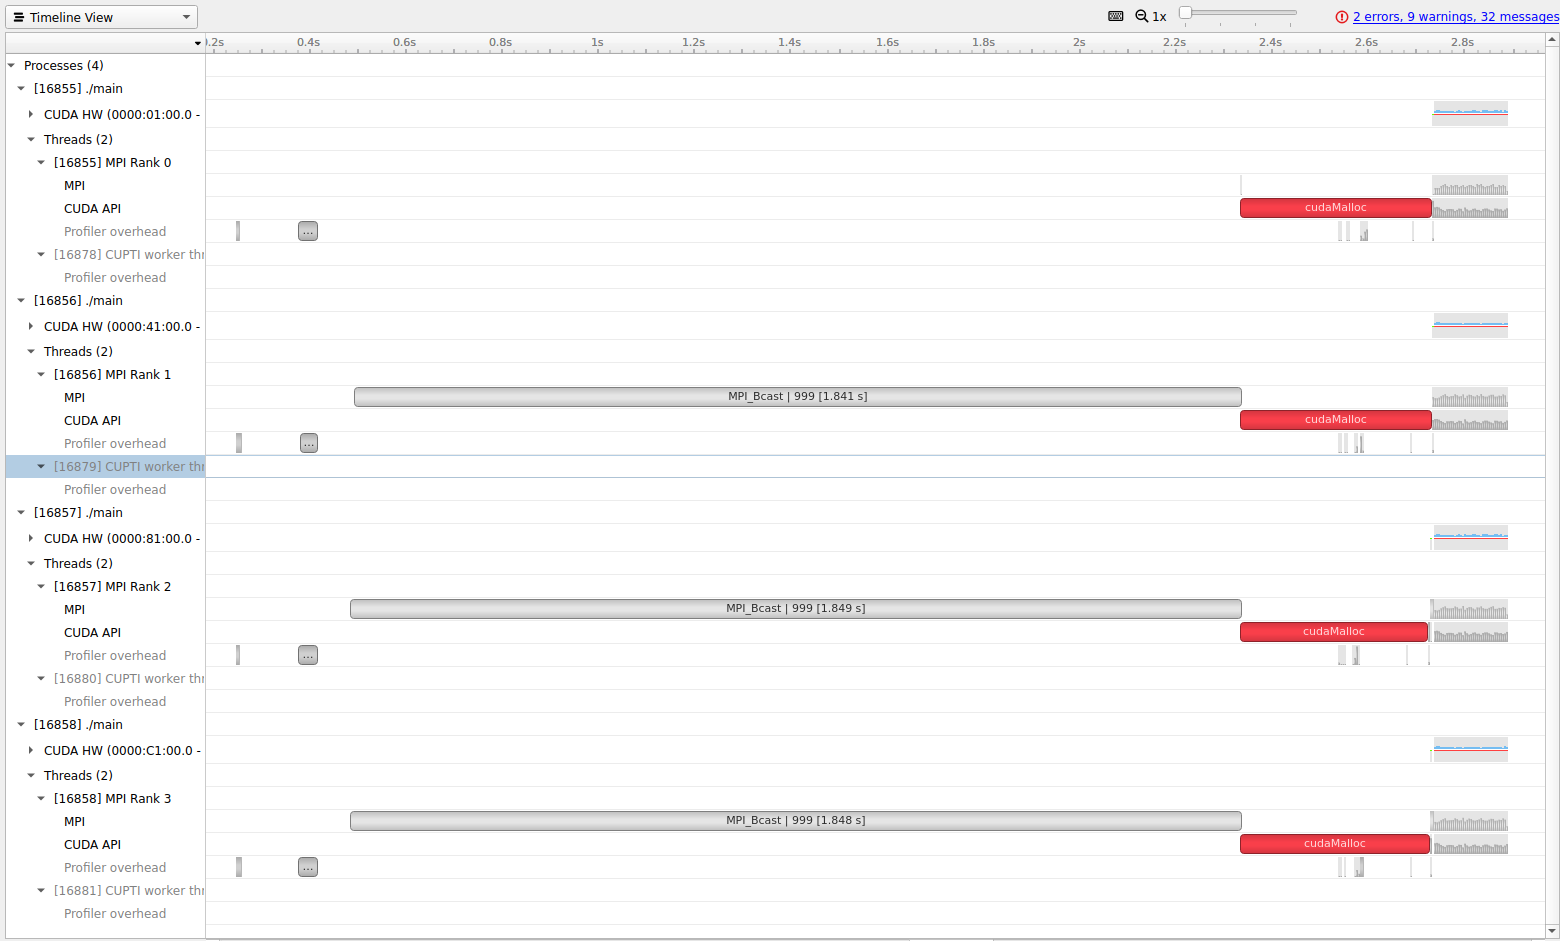
\includegraphics[scale=0.3]{nsight_systems_overview2.png}
    \caption{Nsight Systems timeline of entire program for single epoch}
\end{figure}

Second takeaway (Figure 4) was relative expense of \texttt{MPI\_Scatter} and \texttt{cudaMemcpy}
operations compared with our feed forward, back propagation and gradient descent kernels.
To me this highlights the importance to reducing the number of movements to and from the
device, especially within the batch loops as is currently the case for X and y as well
as gradients pre and post \texttt{MPI\_AllReduce}. A future implementation might consider
splitting work differently across my 4 GPUs (processes) to reduce \texttt{cudaMemcpy} and
\texttt{MPI} statements. Currently I divide each batch into 'mini batches', however,
instead I could think about dividing my model parameters (weights and biases) across
the different processes.

\begin{figure}[!htbp]
    \centering
    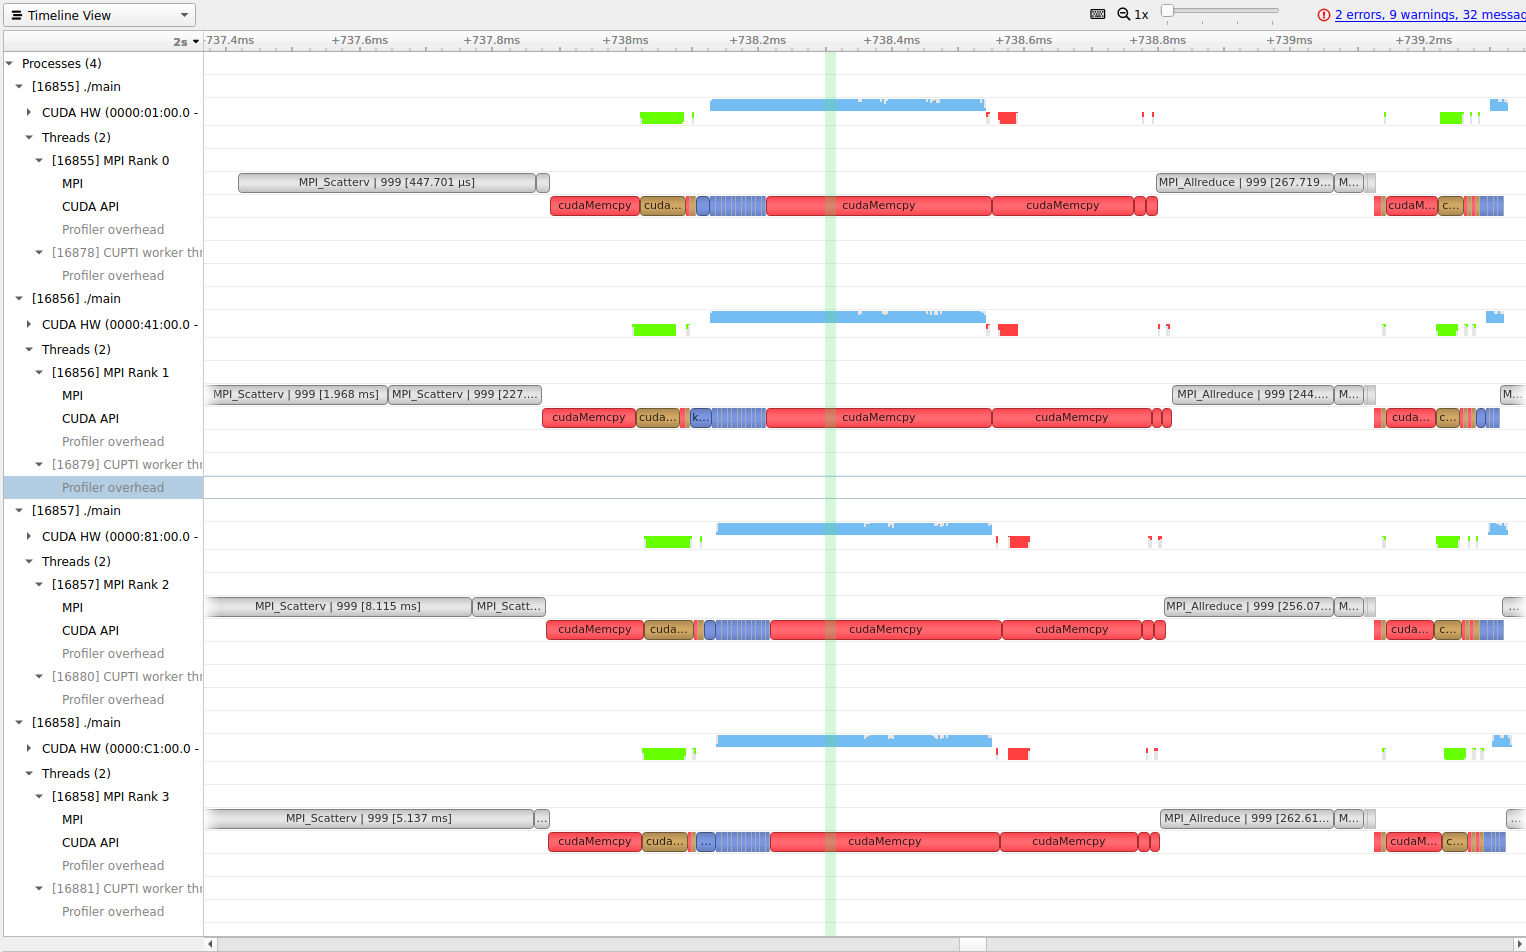
\includegraphics[scale=0.3]{nsight_systems_batch2.png}
    \caption{Nsight Systems timeline for training of one image batch}
\end{figure}

Third takeaway (Figure 5) was that our training pipeline takes noticably (approx. 50\%)
less time for each epoch! This looks to be because (a) we execute far fewer kernels (16
vs 25 for each training cycle), and (b) our GEMM related kernels are all more performant.
This is great news and also agrees with our runtime statistics where updates 1 and 2 made
the largest difference.

\begin{figure}[!htbp]
    \centering
    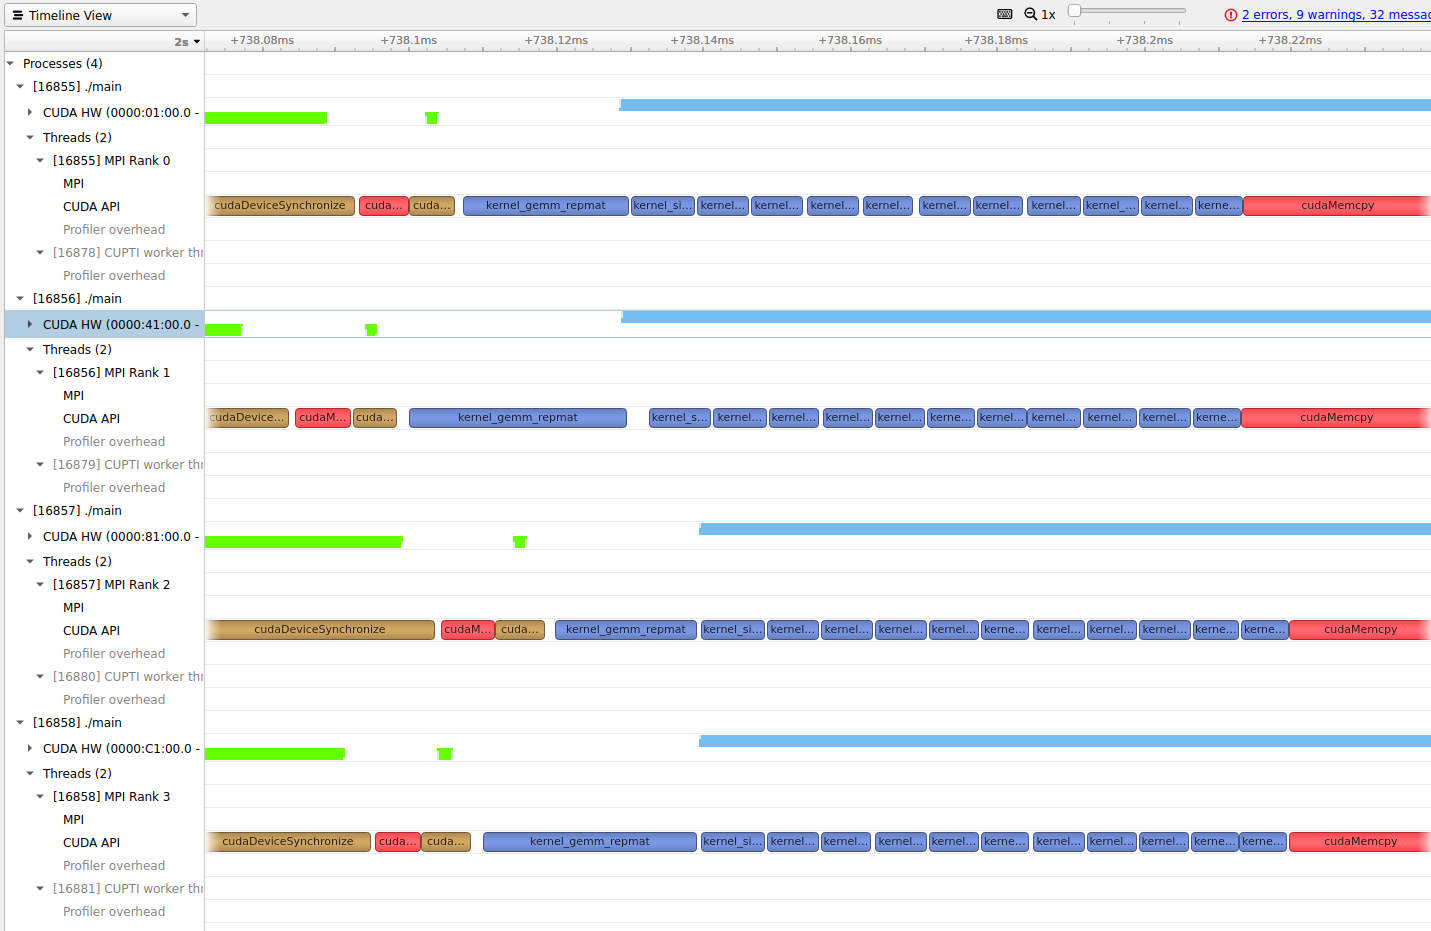
\includegraphics[scale=0.3]{nsight_systems_kernels2.png}
    \caption{Nsight Systems relative time cost of all matrix kernels}
\end{figure}


\textbf{Nsight Compute:} Used to take a deeper look into the performance of
individual kernels for FP32 precision. In particular, our generalized matrix multiplication kernel.

Main takeaway is that we have increased both arithmetic intensity (23.24 FLOP/byte) and performance
($5*10^{9}$ FLOP/sec) significantly compared to our part 1 GEMM implementation! That said, there is still
plenty of performance uplift available as demonstrated in the roofline chart by the gap between
our achieved performance (green dot) and the peak FP32 performancen boundary (top horizontal
blue line). This position implies we are still very much latency bound.

It is intersting to note however that our position in the roofline plot has shifted meaningfully to
the right such that we are no longer near the memory bandwidth bound line. This suggests latency
improvements will contribute directly to improved performance since not constrained immediately
by memory bandwidth.

\begin{figure}[!htbp]
    \centering
    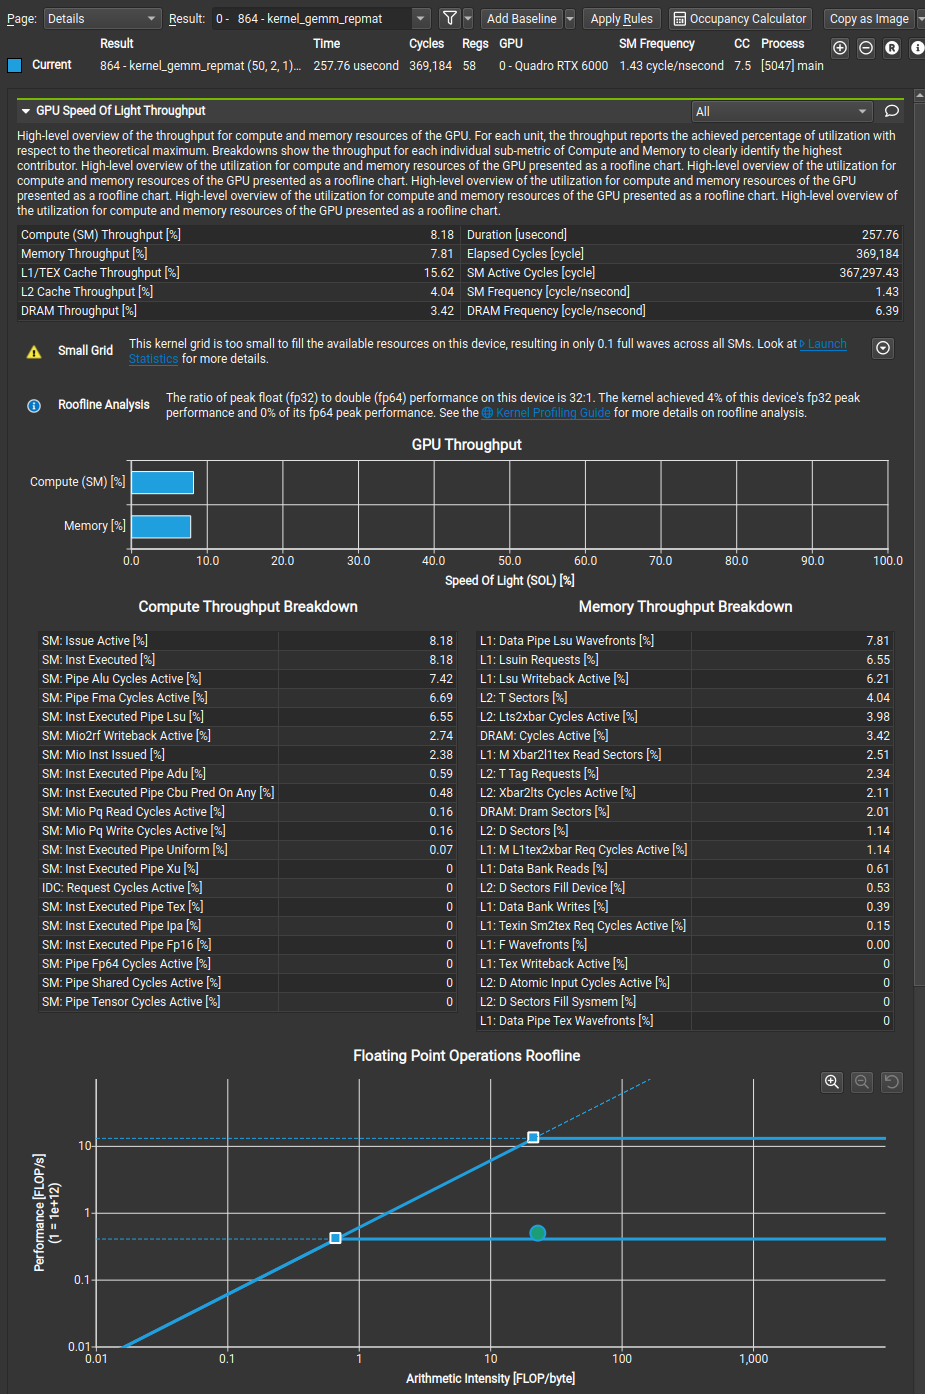
\includegraphics[scale=0.5]{nsight_compute_roofline2.png}
    \caption{Nsight Compute speed of light roofline plot for GEMM kernel}
\end{figure}

Finally, Nsight Compute's launch statistics suggests that I launch too small a grid for the
available hardware specs. Given fixed thread block dimensions and \texttt{numXPerThread},
our grid size is fixed to match the input matrices and so in some sense we are constrained. That
said, it would be interesting to experiment with smaller thread block or \texttt{numXPerThread}
settings that allow for a larger grid and potentially use more of the available hardware
resource at the expense of memory access being less coalesced.

\end{document}
